% Manuel Lippert - Paul Schwanitz
% Physikalisches Praktikum

% Teilaufgabe 3
\newpage
\section{Der Shinriki-Oszillator}
\label{sec:shinrikiOszi}


\subsection{Differentialgleichung und Aufbau des Shinriki-Oszillator}
\label{sub:dgl}

\begin{figure}[h]
    \centering
    %TODO #31
    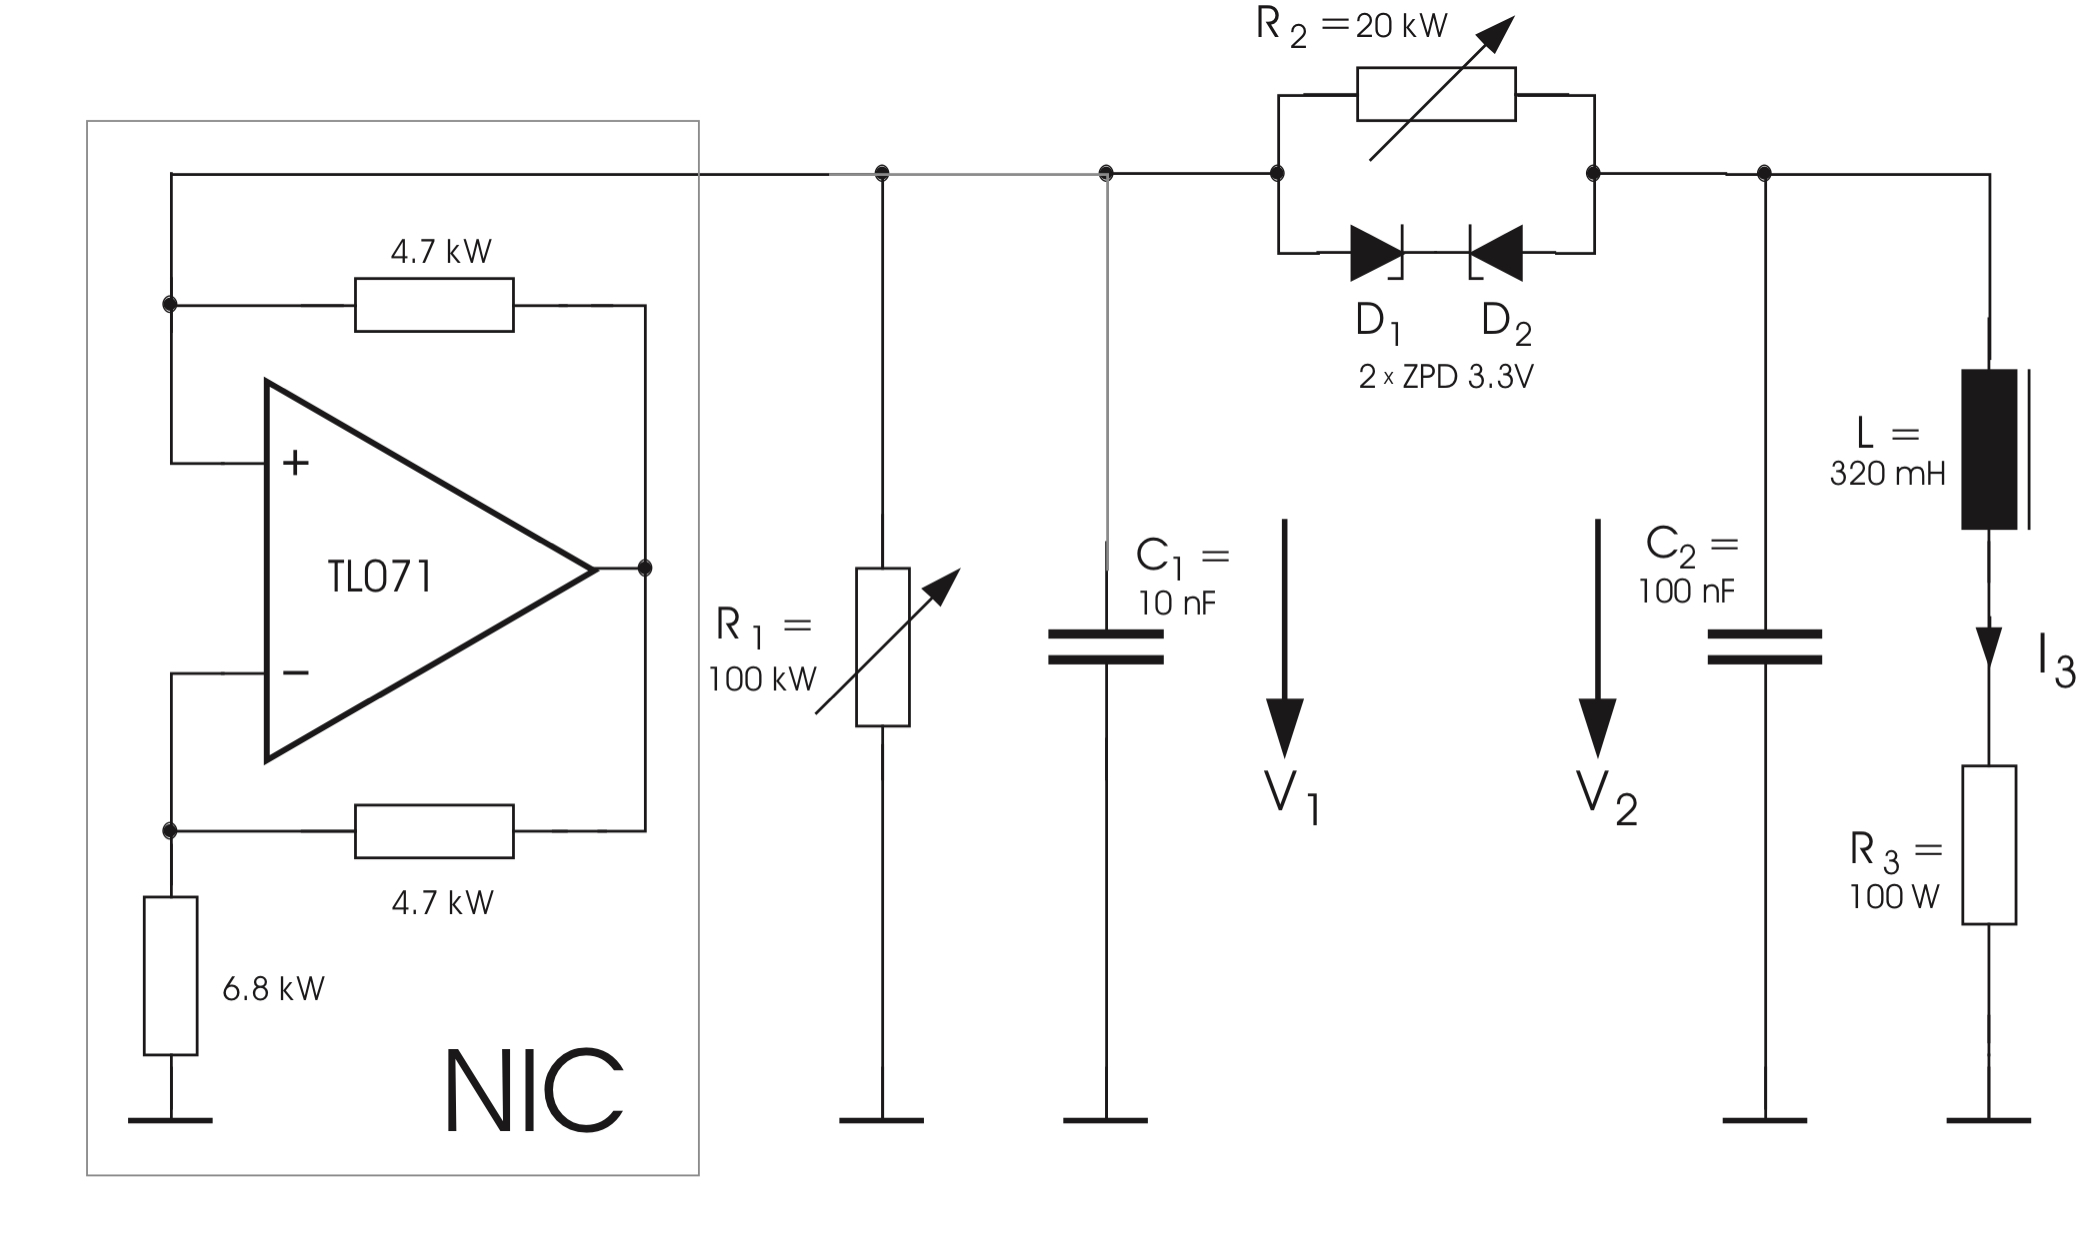
\includegraphics[scale=0.15]{ShinrOsziSp.jpeg}
    \label{fig:shinrikiSp}
    \caption{Schaltplan des Shinriki-Oszilator \citep{Lueck}}
\end{figure}

Der Shinriki-Oszillator besteht aus einem negativen Impedanzkonverter (NIC) und einem LC-Parallelschwinkreis, die durch ein gegeneinader geschaltetes Zenerdiodenpaar und dem parallel geschalteten \(R_2\), gekoppelt sind. \\
Die Leitwertfunktion des Kopplungsglied ist \( f(V)\) und beschreibt den Strom, der über das Kopplungsglied fließt.
\(R_{NIC}\) ist der Widerstand des NIC innerhalb des relevanten Intervalls von -8,1 V bis 8,1 V \citep[]{Lueck}.\\
Damit und mit den Kirchhoffschen Regeln lassen sich nun die DGLs aufstellen:
\begin{align}
    C_1 \dot{V_1} &= V_1 (\frac{1}{R_{NIC}}-\frac{1}{R_1}) - f(V_1-V_2) \\
    C_2 \dot{V_2} &= f(V_1-V_2) - I_3 \\
    L \dot{I_3} &= -I_3R_3 + V_2
\end{align}

\subsection{NIC und Schwingung des Shinriki-Schaltkreis}
\label{sub:nic}
Ein NIC benutzt einen Operationsverstärker, um einen negativen ohmschen Wiederstand zu simulieren. Hierbei wird der gewünschte Widerstand einfach zwischen dem (-) Eingang des OpAmp und GND geschaltet. Durch den OpAmp wird ein Widerstand mit negativem Wert des eben eingesetzten simuliert. \\
Daher mus das System nicht mehr von außen zur Schwingung angeregt werden.
% TODO #29

\subsection{Geräusche einer Bifurkation}
\label{sub:tonBifurkation}
Eine Bifurkation ist eine verdopplung der Periodendauer, d.h. die Frequenz wird halbiert. Dies verursacht einen tieferen Ton.
% TODO #30